\documentclass[10pt,twocolumn]{article}
\usepackage[utf8]{inputenc}
\usepackage[T1]{fontenc}
\usepackage{amsmath,amssymb}
\usepackage{graphicx}
\usepackage{booktabs}
\usepackage[margin=0.8in]{geometry}
\usepackage[numbers]{natbib}
\usepackage{hyperref}

\title{Correcting Weather Forecasts with Learned Token Codebooks}
\author{Test Author\\Texora University}
\date{}

\begin{document}
\maketitle

\begin{abstract}
We basically propose a method that corrects numerical weather forecasts. It uses a codebook and a small network and it works really well on many regions, which is good.
\end{abstract}

\section{Introduction}
\label{sec:intro}
Accurate short-range forecasts matter for agriculture, energy and emergency planning~\cite{lamport1994latex}.
Early methods relied on linear post-processing, while recent work uses deep neural networks~\cite{vaswani2017attention}.

\section{Related Work}
\label{sec:related}

\subsection{Statistical Post-Processing}
Linear corrections are fitted per station and per lead time.

\subsection{Discrete Codebooks and Learned Representations}
Vector-quantised autoencoders learn a discrete codebook of tokens~\cite{knuth1984}.

\subsection{Diffusion Models for Forecasting}
Diffusion models generate sharp fields through iterative denoising~\cite{ho2020denoising}.

\section{Methodology}
\label{sec:method}

\subsection{Overview of the Proposed Framework}
Figure~\ref{fig:plot} gives an overview. The framework has two stages.

\begin{figure}[t]
  \centering
  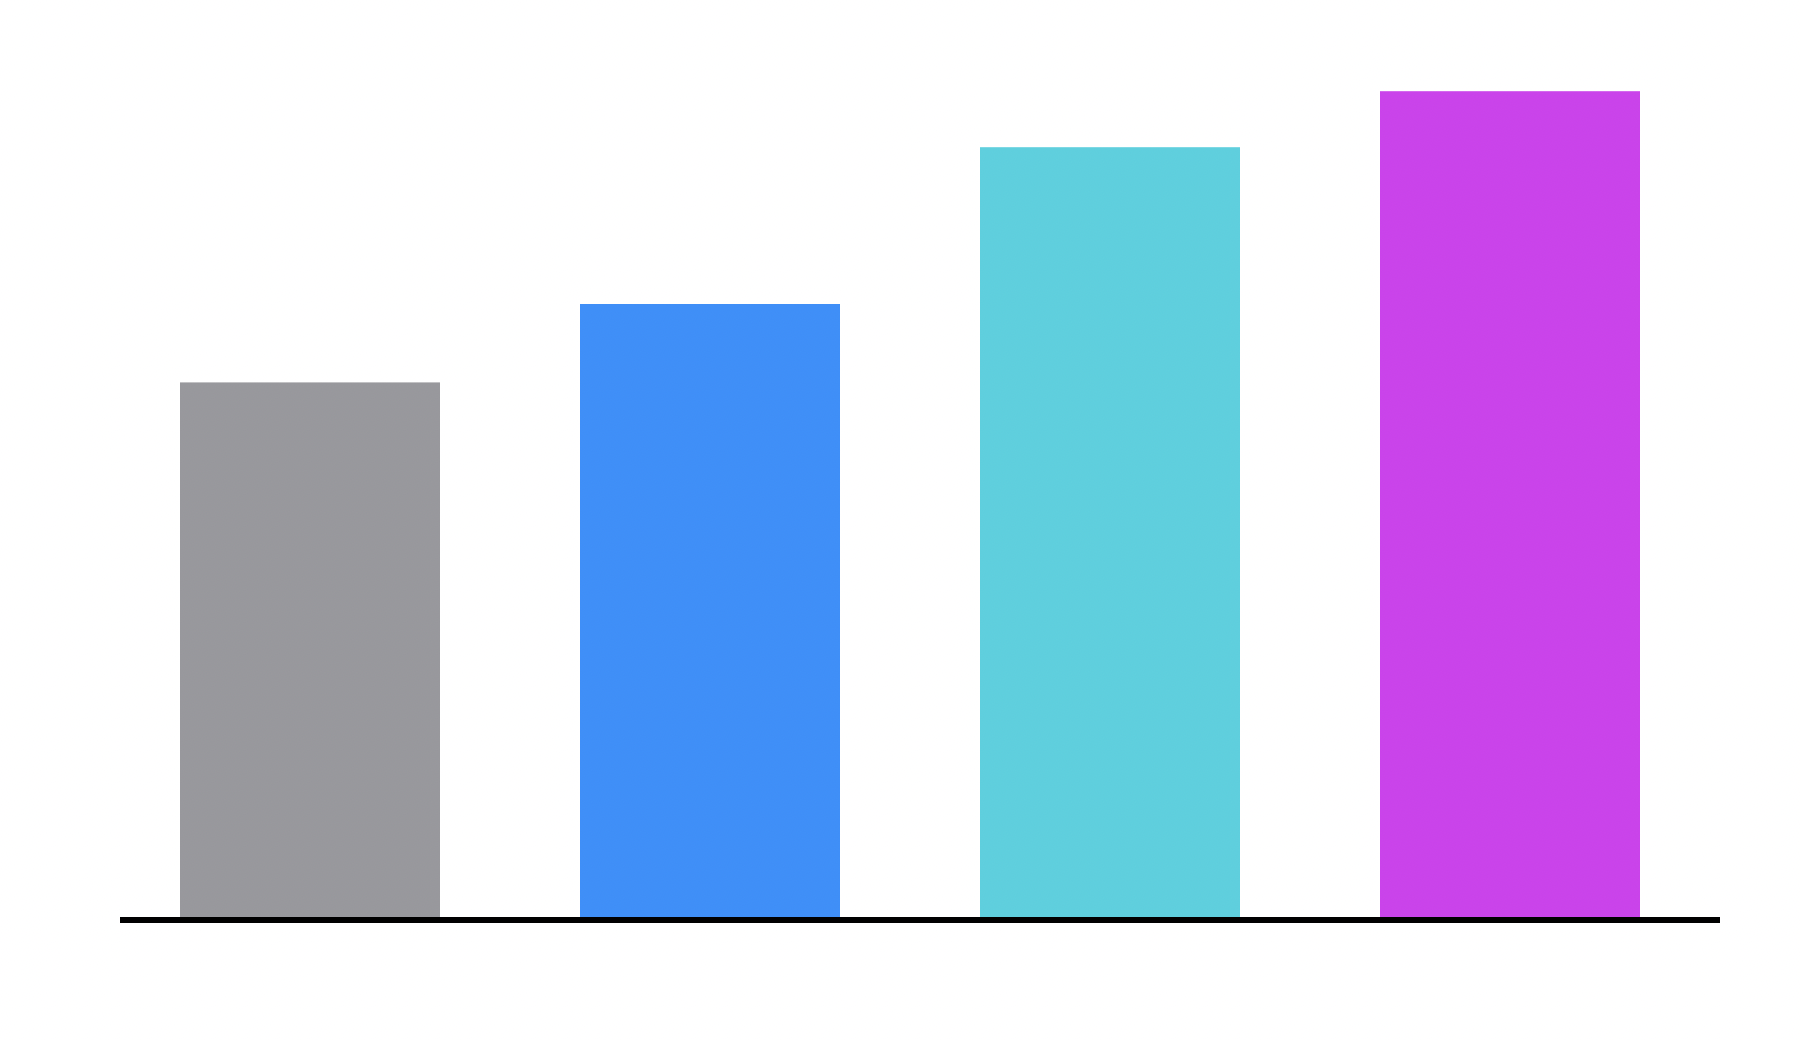
\includegraphics[width=\linewidth]{figures/plot.png}
  \caption{Error reduction of each stage on the validation set.}
  \label{fig:plot}
\end{figure}

\subsection{Notations and Operators}
Let $F$ denote a raw forecast and $O$ the matching observation.

\subsection{Stage 1: Token Codebook}
\subsubsection{Encoder}
The encoder maps the forecast to a latent grid $z = E(F)$.
\subsubsection{Vector Quantization with Dynamic Re-initialization}
Each latent vector is replaced by its nearest codebook entry:
\begin{equation}
  \hat{z}_i = \arg\min_{e_k \in \mathcal{C}} \lVert z_i - e_k \rVert_2 .
  \label{eq:vq}
\end{equation}
\subsubsection{Codebook Training Loss}
We train with the loss in Eq.~\eqref{eq:vq} plus a commitment term.

\subsection{Stage 2: Dual-Path Correction}
\subsubsection{Path 1: Climatology Prior (Fixed)}
A fixed climatology prior supplies seasonal context.
\subsubsection{Path 2: Codebook Tokens $\to$ Correction Head (Trainable)}
A trainable head maps tokens to a residual correction.

\section{Experiments}
\label{sec:results}
Table~\ref{tab:results} reports the main results on the benchmark regions.

\begin{table}[t]
  \centering
  \caption{Comparison with prior methods.}
  \label{tab:results}
  \begin{tabular}{lcc}
    \toprule
    Method & RMSE $\downarrow$ & CRPS $\downarrow$ \\
    \midrule
    Raw forecast & 2.41 & 1.32 \\
    Ours & \textbf{1.62} & \textbf{0.88} \\
    \bottomrule
  \end{tabular}
\end{table}

\section{Conclusion}
We presented a two-stage forecast correction framework.


\bibliographystyle{plainnat}
\bibliography{refs}

\end{document}
